\documentclass[aps, pra, amsfonts, a4paper, showpacs]{revtex4-1}
\usepackage{graphicx,graphics,epsfig}   
\usepackage{dcolumn}    
\usepackage{bm}         
\usepackage{subfigure}  
\usepackage{times,natbib}
\usepackage{amsmath,amsfonts,amssymb,graphics,graphicx,epsfig,color,times,natbib}
\usepackage{xcolor}
\usepackage{braket}
\usepackage{amsmath}
\usepackage{bbold}

\newcommand{\todo}[1]{\textcolor{red}{\texttt{TODO: #1}}}


\begin{document}

\newcommand{\kpz}{\ket{\psi_0}}
\newcommand{\bpz}{\bra{\psi_0}}
\newcommand{\hz}{\braket{H_0}}
\newcommand{\hsqz}{\braket{H^2_0}}
\newcommand{\heff}{H_{\mathrm{eff}}}

\section*{Estimate of Zeno time for hyperfine flip-flops}
Say we start out in a state $\ket{\psi_0}=\ket{\uparrow}\otimes\ket{\phi_0}$, where $\ket{\phi_0}$ is some nuclear state. This is approximately the case after many consecutive cross-polarized detections, which tell us that the nuclear state $\ket{\phi_0}$ is most probably the nuclear state that puts the transition on resonance. 

What is the timescale at which we could Zeno-inhibit the hyperfine evolution (``decay'') of this state? 

\vspace{0.5cm}
Let's start out with the standard expression for the Zeno time $\tau_Z$ \cite{pascazio_all_2014}
\[
\bpz e^{-i H t} \kpz = 1 - i\hz t -\frac{1}{2} \hsqz t^2
\]
where $ \hsqz = \bpz  H^2 \kpz$ and similar for $\hz$.
Then the probability to find the system in state $\kpz$ after a short time $t$ is given by
\begin{equation}
p_0(t) \approx 1- (\hsqz - \hz^2)t^2 \equiv 1- \frac{t^2}{\tau_z^2} 
\label{Eq: p0}
\end{equation}
for $t \ll \tau_Z$.

The full spin Hamiltonian for an external magnetic field along $\hat{z}$ is
\begin{equation}
H=\Omega S^z + \sum_k \omega_k I^z_k + \sum_k A_k I^z_k S^z + \sum_k \frac{A_k}{2}(S^zI^-_k + S^- I_k^+)
\label{Eq: H}
\end{equation}
where the index $k$ runs over all nuclear sites. Denoting the flip-flop term
\[H_{int} = \sum_k \frac{A_k}{2}(S^zI^-_k + S^- I_k^+) \]
and assuming that $\kpz$ be an eigenstate of $H-H_{int}$ one obtains
\begin{equation}
\frac{1}{\tau_z^2} = \sum_n |\braket{\psi_0|H_{int}|\psi_n}|^2
\label{Eq: simp}
\end{equation}
where $\{\ket{\psi_n}\}$ is an orthonormal basis of the electron-nuclear spin system, while $\{\ket{\phi_n}\}$ is a basis of the nuclear system alone.
Assuming the form $\ket{\psi_0}=\ket{\uparrow}\otimes\ket{\phi_0}$ for the initial state, the above expression for $\tau_Z$ simplifies to
\begin{equation}
\begin{split}
\frac{1}{\tau_z^2} &=\sum_n |\braket{\phi_0 | \sum_k \frac{A_k}{2} I_k^+ |\phi_n}|^2 \\
&= \sum_k \sum_l \frac{A_k A_l}{4}\braket{\phi_0 | I_k^+ I_l^- |\phi_0} \\
&= \sum_k \frac{A_k^2}{4}(J_k(J_k+1) - m_k(m_k -1)).
\end{split}
\end{equation}
Here the numbers $m_k$ ($J_k$) denote the z-component (maximum projection) of the $k$th spin in the initial nuclear state $\ket{\phi_0}$.

Let's talk about two questions:
\begin{itemize}
\item Can we measure fast enough for a realistic distribution $\{A_k\}$?
\item How do we tell if we observe this Zeno effect or not?
\end{itemize}

We address the first question by computing values of $\tau_Z$ for a range of coupling strength distributions $\{ A_k \}$. Taking $\hat{z}$ along the growth axis of the quantum dot, we assume that the wavefunction follows a Gaussian distribution with a cutoff in the $x-y$ plane and is constant along $\hat{z}$. There are three parameters to describe such a distribution: the radius in the $x-y$ plane beyond which we set the coupling to zero is denoted $r$. The number of atomic layers in the $\hat{z}$ direction is $N_z$ and the decay constant is denoted $R$. Hence
\begin{equation}
A_{(x,y)}=\frac{A_{tot}}{N_z}\frac{\exp(-\alpha(x^2+y^2))m_{(x,y)}}{\sum_{(x,y)}\exp(-\alpha(x^2+y^2))m_{(x,y)}}
\label{Eq: dist}
\end{equation}
where
\[\begin{split}
m_{(x,y)}&= 1\ \  \mathrm{for}\ x^2+y^2<r^2 \\
 &= 0\ \  \mathrm{else}
\end{split}\] and where the indices $x,y$ take on integer values.
We assume nuclear spin $J_k=\frac{1}{2}$ and a nuclear state in which the flipable spins are uniformly distributed. Furthermore take $N_z=10$.
The plots presented in Fig. \ref{Fig: tz} show that Zeno times seem to lie in the nanosecond regime under these assumptions.

\begin{figure}
    \centering
    \begin{minipage}{.45\textwidth}
        \centering
        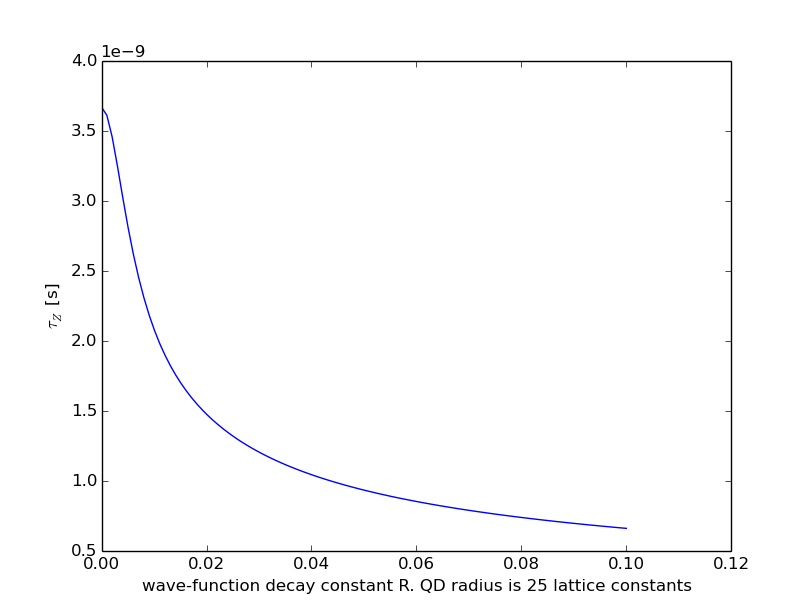
\includegraphics[width=\linewidth]{tz_vs_R.png}
        \caption{Zeno time vs. decay constant $R$ at a radius $r=25$.}
    \end{minipage}%
    \begin{minipage}{0.45\textwidth}
        \centering
        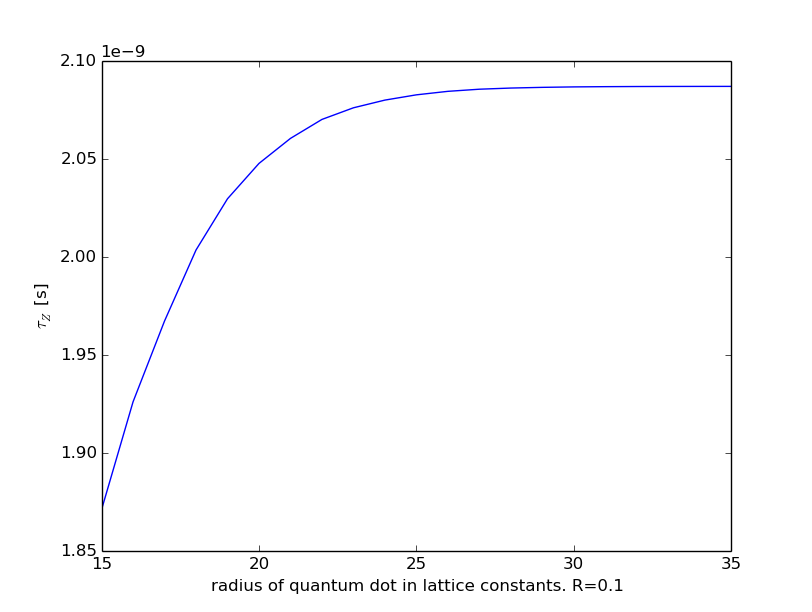
\includegraphics[width=\linewidth]{tz_vs_radius.png}
        \caption{Zeno time vs. cutoff radius $r$ for decay constant $R=0.1$.}
    \end{minipage}
    \label{Fig: tz}
\end{figure}


\section*{Estimate of Zeno time for the Overhauser field with constant electron spin polarization}
Given a Zeeman splitting of the electron spin states much larger than the hyperfine interaction energy, flip-flops of the electron spin with nuclei occur with small probability amplitude. The hyperfine interaction in this regime is to a good approximation of pure dephasing character. Approximating a hyperfine Hamiltonian by a pure dephasing Hamiltonian involves replacing the electron-nuclear flip-flop terms $S^+I_k^- + S^-I_k^+$ by electron mediated nucleus-nucleus flip-flop terms of the form $S^Z(I_k^+I_l^- + I_k^-I_l^+$.

A pure dephasing Hamiltonian can describe electron spin decoherence, which has been studied in \cite{cywinski_electron_2009} and others. It also provides a microscopic model of the quantum dynamics underlying Overhauser field fluctuations. These quantum dynamics have been recognized in \cite{klauser_nuclear_2008} to possibly enable experimental observation of a Zeno effect. However measurement of the Overhauser field with sufficient accuracy and speed has been a daunting task, up until the arrival of the low-Q QD cavity phase shift thing.

In the following we study the dynamics of the pure dephasing Hamiltonian presented in \cite{klauser_nuclear_2008} in order to estimate the Zeno time of the Overhauser field and make experimentally verifiable predictions about its behaviour. The effective Hamiltonian can be writen as $\heff=H_0 + V$, where
\begin{equation}
\begin{split}
H_0 &= \epsilon S^z + \eta_z \sum_k I_k^z + S^z \sum_k A_k I_k^z \\
V &= \frac{1}{2\omega} (S^z \sum_{k \neq l} A_k A_l I_k^+ I_l^- + \frac{1}{2}\sum_k A_k^2(S^z - I_k^z)),
\end{split}
\label{Eq: Heff}
\end{equation}
which is valid for $I_k = \frac{1}{2}$ and $\frac{1}{\omega}$ with $\omega=\epsilon_z - \eta_z + \braket{\sum_kA_kI_k^z}$ approximately constant.

Note that this Hamiltonian commutes with $S^z$ as well as $\sum_k I_k^z$, which means that its eigenstates live in subspaces of fixed $\sum_k I_k^z$ and fixed electron spin projection. So rather than diagonalizing a matrix of dimension $2^{N+1}$ (N number of nuclear spins) we have to deal with (still bloody big) blocks of dimension 
\[
\sum_{i=0}^{\min\{n_{\downarrow},n_{\uparrow}\}} \binom{n_{\uparrow}}{i}\binom{n_{\downarrow}}{i},
\]
where $\braket{\sum_kI_k^z} = \frac{1}{2}(n_{\uparrow}-n_{\downarrow})$.

The effective Hamiltonian can be written as 
\begin{equation}\begin{split}
&\heff =S^z \otimes \hat{A} + \mathbb{1} \otimes \hat{B} \\
&\mathrm{where\ the\ nuclear\ operators\ are}\\
&\hat{A}=(\epsilon_z + \frac{1}{4\omega}\sum_k A_k^2)\mathbb{1} + \sum_k A_k I_k^z + \frac{1}{2\omega}\sum_{k \neq l} A_k A_l I_k^+ I_l^- \\
&\hat{B} = \eta_z \sum_k I_k^z - \frac{1}{4\omega} \sum_k A_k^2 I_k^z.
\end{split} \label{Eq. AB} \end{equation}

Since the laser couples the electron states $\ket{\uparrow}$, $\ket{\downarrow}$ to the trion states it is the spectrum of the nuclear operator $\hat{A}$ that determines the detuning of the transition and thereby the phase shift of a photon. The eigenstates $\ket{a}$ of $\hat{A}$ are the states which lead to a definite phase shift and are therefore suitable for an electron spin-photon entangling operation, while superpositions of different nuclear states $\ket{A}$ can lead to nuclear spin - photon entanglement.

The spectrum and eigenstates of $\hat{A}$ are generally not tractable. However there are certain simple cases which can be studied analytically and which can serve to illustrate qualitative features of the model and help to understand numerical results presented later on. We present the perturbative analysis of the graded box model \cite{petrov_coupled_2009}, which assumes that all nuclear couplings take on one of two different coupling strengths:
\begin{equation}\begin{split}
A_k &= A_1\ \ \ \mathrm{for}\ 1 \leq k \leq N_1\\ 
A_k &= A_2\ \ \ \mathrm{for}\ N_1+1 \leq k \leq N.
\end{split} \label{Eq: A graded} \end{equation}

The nuclear operators become
\begin{equation}\begin{split}
\hat{A}&=\epsilon_z \mathbb{1} + A_1 I_1^z + A_2 I_2^z + \frac{1}{2\omega}\left(A_1^2 (I_1^2 - (I_1^z)^2) + A_2^2 (I_2^2 - (I_2^z)^2 ) + A_1 A_2 (I_1^+ I_2^- + I_1^- I_2^+)\right) \\
\hat{B}&=\eta_z(I_1^z + I_2^z) -  \frac{1}{4\omega}(A_1^2 I_1^z + A_2^2 I_2^z)
\end{split} \label{Eq: H graded}
\end{equation}
where
\[
I^{z/+}_1 = \sum_{k=1}^{N_1} I_k^{z/+} \hspace{0.5cm} ,\hspace{0.5cm} I^{z/+}_1 = \sum_{k=N_1+1}^{N} I_k^{z/+}.
\]
The identity $I^+I^-=I^2 - (I^z)^2 + I^z$ has been used in going from Eq. \ref{Eq: Heff} to Eq. \ref{Eq: H graded}. Note that the nuclear operators are tridiagonal in the basis of eigenstates of the operators $I_1^2, I_2^2, I_1^z, I_2^z$, which are introduced in \cite{petrov_coupled_2009} and \cite{kozlov_exactly_2007}. 

\subsection*{Perturbative analysis of the Overhauser Zeno time}
We would like to know the spectrum of $\hat{A}$, which will correspond to the possible transition energies. Since the phase shift is a function of the detuning, a nuclear spin system in an eigenstate $\ket{a}$ of $\hat{A}$ will lead to a definite phaseshift $\theta$ on a scattered photon:
\[
\ket{\downarrow}_e \otimes \ket{a}_n \otimes \ket{V}_p \xrightarrow{scatter} \ket{\downarrow}_e \otimes \ket{a}_n \otimes \ket{\theta(a)}_p,
\]
where the subscripts $e$, $n$, $p$ denote electron, nuclei, and photon, respectively.

The almost diagonal form of $\hat{A}$ in the graded box model approximation (Eq. \ref{Eq: H graded}) suggests time-independent nondegenerate perturbation theory. We therefore write
\[
\hat{A} = A_0 + A^{(1)}\] where
\[ A^{(1)} = \frac{A_1A_2}{2\omega}(I_1^+ I_2^- + I_1^- I_2^+).\]
The unperturbed states are the eigenstates of $I_1^2, I_2^2, I_1^z, I_2^z$:
\[
 A_0 \ket{\psi}_0 = A_0 \ket{I_1,I_2,m_1,m_2} = \left( A_1m_1 + A_2 m_2 - \frac{1}{2\omega}(A_1^2 m_1^2 + A_2^2 m_2^2) \right) \ket{I_1,I_2,m_1,m_2} = E_{m1,m2}^{(0)}\ket{\psi}_0
\]
where we have omitted the constant transition energy $\epsilon_z$.

Since each state $\ket{I_1,I_2,m_1,m_2}$ only couples to two other states $\ket{I_1,I_2,m_1+1,m_2-1}$ and $\ket{I_1,I_2,m_1-1,m_2+1}$ under $A^{(1)}$, the second-order correction to the transition energy and first-order correction to the state $\ket{a}$ are readily computed:
\begin{equation}\begin{split}
E_{m_1,m_2}^{(2)}&=\frac{(A_{+-}^{m_1,m_2})^2}{E_{m_1,m_2}^{(0)} - E_{m_1+1,m_2-1}^{(0)}} + \frac{(A_{-+}^{m_1,m_2})^2}{E_{m_1,m_2}^{(0)} - E_{m_1-1,m_2+1}^{(0)}} \\
\ket{\psi_{m_1,m_2}^{(1)}}&=\frac{A_{+-}^{m_1,m_2}}{E_{m_1,m_2}^{(0)} - E_{m_1+1,m_2-1}^{(0)}} \ket{m_1 + 1, m_2 - 1} + \frac{A_{-+}^{m_1,m_2}}{E_{m_1,m_2}^{(0)} - E_{m_1-1,m_2+1}^{(0)}}\ket{m_1 - 1, m_2 + 1}
\end{split} \label{Eq: corrections}
\end{equation}
with 
\[
A_{+- / -+}^{m_1, m_2}=\frac{1}{2\omega}A_1A_2\sqrt{I_1(I_1+1)-m_1(m_1 \pm 1)}\sqrt{I_2(I_2+1)-m_2(m_2 \mp 1)}
\]

We now calculate the Zeno time of the states $\ket{a^{(1)}}=N(\ket{\psi}_0 + \ket{\psi^{(1)}})$:
\[ \frac{1}{\tau_z^{(1)}} = \braket{a^{(1)} | \hat{B}^2 | a^{(1)}} - (\braket{a^{(1)} | \hat{B} | a^{(1)}})^2. \]
This timescale has the following interpretation:
Assume that the nuclear system can be initialized in a phase eigenstates $\ket{a}$. This could approximately be achieved by a large number of consecutive cross-polarized counts, making it overwhelmingly likely that the nuclear bath is in the state $\ket{a_{res}}$ that puts the transition in resonance with the laser. The states $\ket{a}$, however, are not energy eigenstates of the full nuclear Hamiltonian $\hat{A} + \hat{B}$. The state $\ket{a}$ evolves under the propagator $\exp^{-i \hat{B} t}$. This evolution is initially described by
\[
|\braket{a | \exp^{-i \hat{B} t} | a}|^2 =1- \frac{t^2}{\tau_Z^2} 
\]
The first-order approximation $\tau_Z^{(1)}$ of this timescale is shown in Fig. \ref{fig: tz} as a plot against Zeeman splitting $\omega$. For $\omega=10\mu \mathrm{eV}$ ($\omega=100 \mu \mathrm{eV}$) the Zeno time approximates to $\tau_Z=8 \mathrm{ms}$ ($\tau_Z=415 \mathrm{ms}$).

\begin{figure}
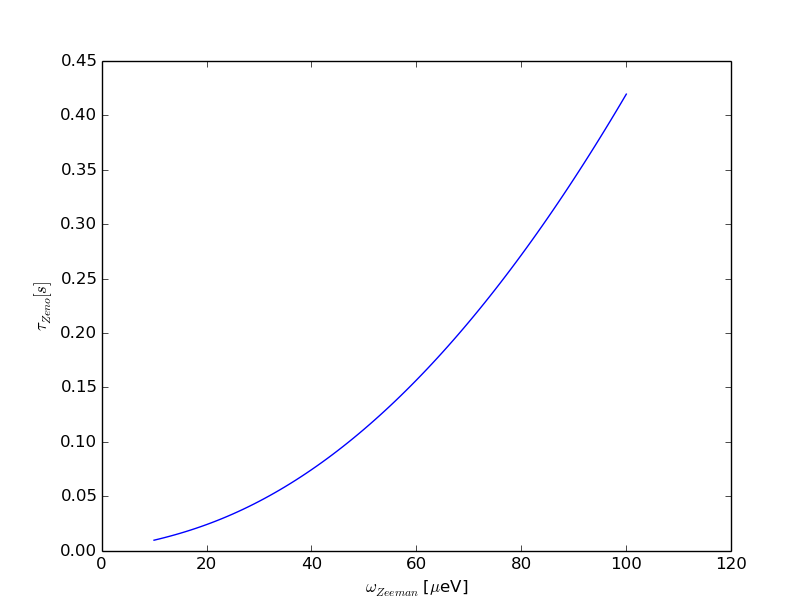
\includegraphics[width=0.6\linewidth]{zeno_redistribution.png}
\label{fig: tz}
\end{figure}

One might therefore hope to observe this suppression of Overhauser field drift by the external magnetic field as increase of average cross-count plateau duration with the Zeeman splitting. baba

\bibliography{Refs_zeno}
\end{document}